\newtcolorbox{taxobox}[1][]{
  enhanced,
  colback=sntPurple!5,
  colbacktitle=sntPurple,
  coltitle=white,
  sharp corners,
  frame hidden,
  boxrule=0pt,
  fontupper=\small,
  fonttitle=\centering\bfseries\scshape,
  after title app=\strut,
  height=3.5cm,
  title=#1
}

\subsection[\eiffel Assessment \& \texttt{eiffel}]{\texorpdfstring{\eiffel Assessing the Impact of Label-Flipping Attacks}{Assessing the Impact of Label-Flipping Attacks}}


% \begin{frame}[plain]
%   \subsectionpage

%   \footcite*{lavaur_ares_bass_2024}
%   \footcite*{lavaur_cose_2025}
% \end{frame}


\begin{frame}{The Problem of Poisoning Attacks}
  \stepcounter{beamerpauses}
  \begin{columns}
    \column{.5\textwidth}
      \begin{block}{Definition}
        Manipulation of the training data or model updates cause unwanted behaviors in the aggregated model.
      \end{block}
      \onslide<+->{
      \begin{block}{Unclear impact in FIDSs}
        \begin{itemize}
          \item Big systematic study on characterizing label-flipping attacks in FIDSs~\autocite{lavaur_cose_2025}.
          \item Scope: predictability, hyperparameter dependencies, impact characterization and detection.
          \item Reproducible evaluation framework (\texttt{eiffel}).
        \end{itemize}
      \end{block}
      }
      
    \column{.5\textwidth}
      \onslide<1->{
      \begin{figure}
        \centering
        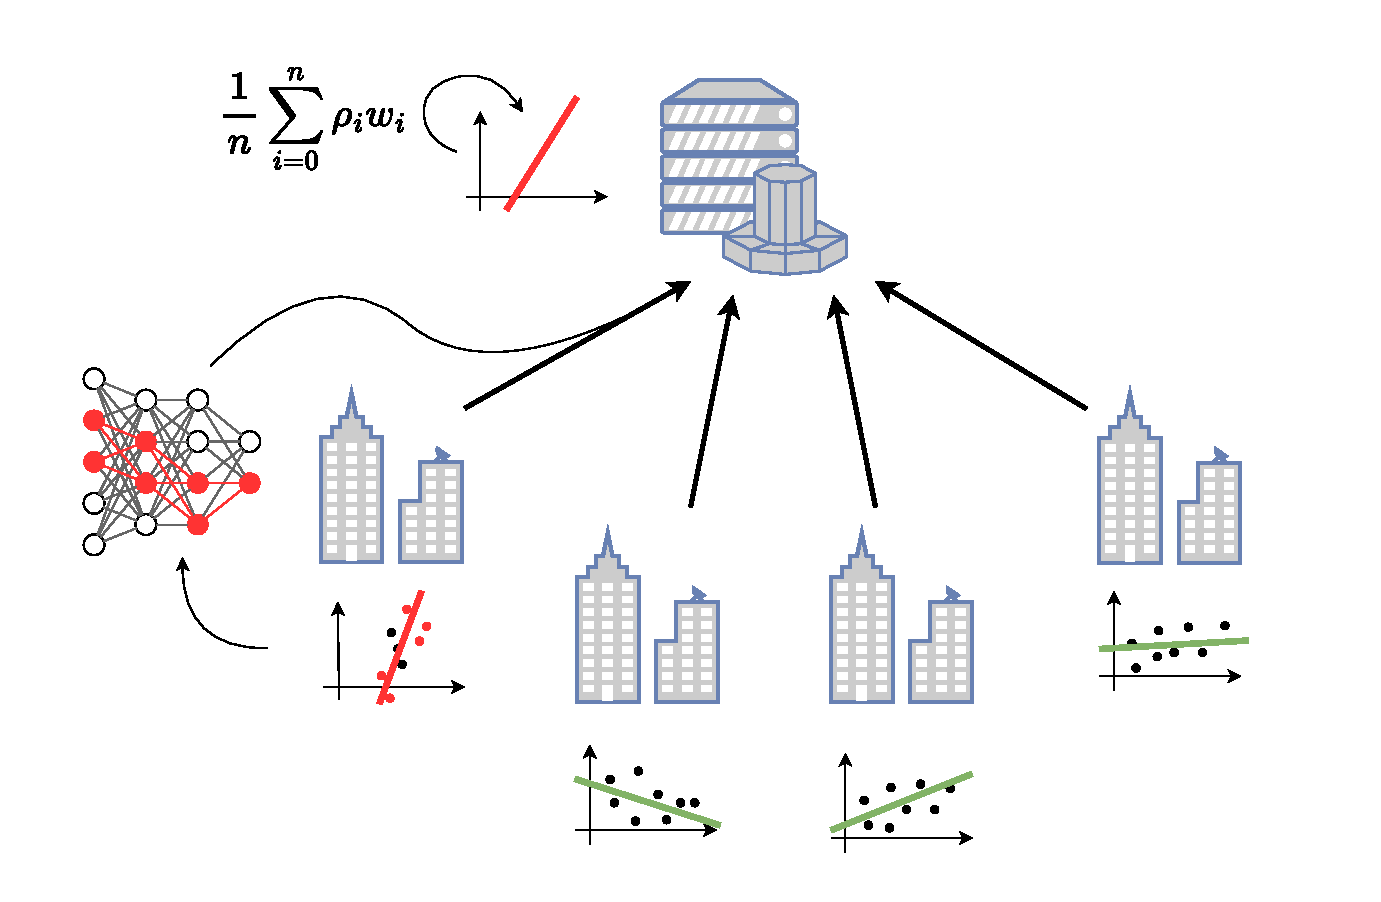
\includegraphics[width=\textwidth,trim={0 1cm 0 1cm},clip]{figures/thesis/assessment/poisoning/6.pdf}
        \caption{Poisoning attacks on FL.}
      \end{figure}}
  \end{columns}

  \alt<2->{\footcite*{lavaur_cose_2025}}{\blankfootnote{\newline}}
\end{frame}

% \begin{frame}{Characterizing Poisoning Attacks}
%   \centering
%   \begin{tcolorbox}[
%     enhanced,
%     colback=sntBlue,
%     boxrule=0pt,
%     frame hidden,
%     fontupper=\large\bfseries,
%     hbox,
%     colupper=white,
%   ]
%     Poisoning attacks
%   \end{tcolorbox}
  
%   \vspace{1em}
  
%   \setlength{\leftmargini}{5pt}
%   \begin{columns}
%     \pause\column{.33\textwidth}
%     \begin{taxobox}[Component]
%       \begin{itemize}
%         \item Data poisoning (\eg, \alert<5>{label-flipping}, clean-label)
%         \item Model poisoning (\eg, gradient boosting)
%       \end{itemize}
%     \end{taxobox}

%     \pause\column{.33\textwidth}
%     \begin{taxobox}[Objective]
%       \begin{itemize}
%         \item Untargeted: impact model performance
%         \item Targeted: modify behavior for specific samples
%       \end{itemize}
%     \end{taxobox}

%     \pause\column{.33\textwidth}
%     \begin{taxobox}[Proportion]
%       \begin{itemize}
%         \item Single attacker
%         \item Colluding attackers: multiple coordinated adversaries
%       \end{itemize}
%     \end{taxobox}
%   \end{columns}
% \end{frame}
  

% \begin{frame}{Scope of the Study}
%   \textbf{Existing studies}
%   \begin{itemize}
%     \item Often partial, focusing on challenging a specific defense mechanism.
%     \item Lack of reproducibility and comparability (different datasets, models, and attacks).
%     \item No targeted attacks binary classification.
%   \end{itemize}

%   % \pause
%   % \textbf{Research Questions}
%   % \begin{enumerate}
%   %   \item Is the behavior of poisoning attacks predictable?
%   %   \item Do hyperparameters influence the impact of poisoning attacks?
%   %   \item Are IDS backdoors realistic using label-flipping attacks?
%   %   \item Is there a critical threshold where label-flipping attacks begin to impact performance?
%   %   \item \alert<3>{Is gradient similarity enough to detect label-flipping attacks?}
%   % \end{enumerate}
% \end{frame}


\begin{frame}{Similarity-based Mitigation against Heterogeneity}

  \begin{columns}
    \begin{column}{.45\textwidth}
      \begin{itemize}[<+->]
        \item Known technique to detect poisoning attacks~\autocite{tolpegin_DataPoisoningAttacks_2020}.
        \item High heterogeneity makes it harder to detect attackers.
      \end{itemize}
    \end{column}

    \begin{column}{.55\textwidth}
      \begin{figure}
        \centering
        \foreach \i in {1,...,3}{%
          \includegraphics<\i>[width=\textwidth,trim={1cm 3cm 1cm 3cm},clip]{figures/thesis/assessment/similarity-untargeted-colluding-cicids-\i.pdf}%
        }
        \caption{PCA projection of the gradients in 2D (CICIDS).}
      \end{figure}
    \end{column}
  \end{columns}

  \footcite*{tolpegin_DataPoisoningAttacks_2020}

\end{frame}

% \begin{frame}{Highlights}
%   % \begin{enumerate}
%   %   \item A \emph{deeper} understanding of the behavior of label-flipping attacks in FL-based CIDSs.

%   \begin{block}{Detection using similarity is not enough}
%     Increasing \alert{heterogeneity} removes the baseline necessary to discriminate contributions
%   \end{block}

%   \pause
%   \begin{block}{Good generalizability defeat tageted poisoning}
%     Feature-overlap between classes and model's \alert{generalization} capabilities limit the attacker's ability to select specific attack classes.
%   \end{block}

%   \pause
%   \begin{block}{High hyperparameter depdendencies}
%     Hyperparameter choices have a significant impact on the attack's impact and \alert{propagation}.
%   \end{block}

%   \footcite*{lavaur_cose_2025}
  
% \end{frame}